%%=============================================================================
%% Proof-of-concept
%%=============================================================================

\chapter{\IfLanguageName{dutch}{Bijlagen}{Attachments}}%
\label{ch:Bijlagen}

\section{Voorbeeldapplicatie}
Hier is een meer gedetailleerd stappenplan terug te vinden met extra informatie of afbeeldingen om de voorbeeldapplicatie te maken.

\paragraph{Stap 1: Maak een secret genereerder door middel van een kustomization bestand}
Door het volgend commando uit te voeren wordt er een kustomization.yaml bestand aangemaakt die een secret aanmaakt van een gekozen wachtwoord.
\begin{lstlisting}[language=tex, caption={Maak een secret genereerder door middel van een kustomization bestand}]
cat <<EOF >./kustomization.yaml
secretGenerator:
- name: mysql-pass
  literals:
   - password=arno
EOF
\end{lstlisting}

\paragraph{Stap 2: Bronconfiguratie toevoegen voor MySQL en WordPress}
In deze stap wordt er een MySQL database ontplooit. De MySQL container. De MySQL-container koppelt het PersistentVolume op \textit{/var/lib/mysql}. De \textit{MYSQL\_ROOT\_PASSWORD} omgevingsvariabele stelt het databasewachtwoord van het Secret in.

Er word een \textit{mysql-deployment.yaml} bestand aangemaakt met onderstaande code.
\begin{lstlisting}[language=tex, caption={Configuratie mysql}]
apiVersion: v1
kind: Service
metadata:
  name: wordpress-mysql
  labels:
    app: wordpress
spec:
  ports:
    - port: 3306
  selector:
    app: wordpress
    tier: mysql
  clusterIP: None
---
apiVersion: v1
kind: PersistentVolumeClaim
metadata:
  name: mysql-pv-claim
  labels:
    app: wordpress
spec:
  accessModes:
    - ReadWriteOnce
  resources:
    requests:
      storage: 20Gi
---
apiVersion: apps/v1
kind: Deployment
metadata:
  name: wordpress-mysql
  labels:
    app: wordpress
spec:
  selector:
    matchLabels:
      app: wordpress
      tier: mysql
  strategy:
    type: Recreate
  template:
    metadata:
      labels:
        app: wordpress
        tier: mysql
    spec:
      containers:
      - image: mysql:5.6
        name: mysql
        env:
        - name: MYSQL_ROOT_PASSWORD
          valueFrom:
            secretKeyRef:
              name: mysql-pass
              key: password
        ports:
        - containerPort: 3306
          name: mysql
        volumeMounts:
        - name: mysql-persistent-storage
          mountPath: /var/lib/mysql
      volumes:
      - name: mysql-persistent-storage
        persistentVolumeClaim:
          claimName: mysql-pv-claim
\end{lstlisting}

Het volgende bestand is \textit{wordpress-deployment.yaml}. Dat bestand ontplooit een wordpress container en koppelt het PersistentVolume aan \textit{/var/www/html} voor website data bestanden. De \textit{WORDPRESS\_DB\_HOST} omgevingsvariabele stelt de naam van de hierboven gedefinieerde MySQL Service in, en WordPress zal de database aanspreken via de Service. De \textit{WORDPRESS\_DB\_PASSWORD} omgevingsvariabele stelt het databasewachtwoord in van het door kustomize gegenereerde Secret.

\begin{lstlisting}[language=tex, caption={Configuratie wordpress}]
apiVersion: v1
kind: Service
metadata:
  name: wordpress
  labels:
    app: wordpress
spec:
  ports:
    - port: 80
  selector:
    app: wordpress
    tier: frontend
  type: LoadBalancer
---
apiVersion: v1
kind: PersistentVolumeClaim
metadata:
  name: wp-pv-claim
  labels:
    app: wordpress
spec:
  accessModes:
    - ReadWriteOnce
  resources:
    requests:
      storage: 20Gi
---
apiVersion: apps/v1
kind: Deployment
metadata:
  name: wordpress
  labels:
    app: wordpress
spec:
  selector:
    matchLabels:
      app: wordpress
      tier: frontend
  strategy:
    type: Recreate
  template:
    metadata:
      labels:
        app: wordpress
        tier: frontend
    spec:
      containers:
      - image: wordpress:4.8-apache
        name: wordpress
        env:
        - name: WORDPRESS_DB_HOST
          value: wordpress-mysql
        - name: WORDPRESS_DB_PASSWORD
          valueFrom:
            secretKeyRef:
              name: mysql-pass
              key: password
        ports:
        - containerPort: 80
          name: wordpress
        volumeMounts:
        - name: wordpress-persistent-storage
          mountPath: /var/www/html
      volumes:
      - name: wordpress-persistent-storage
        persistentVolumeClaim:
          claimName: wp-pv-claim  
\end{lstlisting}

Deze bestanden worden toegevoegd worden aan de \textit{kustomization.yaml} met volgend commando.
\begin{lstlisting}[language=tex, caption={Kustomization.yaml}]
cat <<EOF >>./kustomization.yaml
resources:
  - mysql-deployment.yaml
  - wordpress-deployment.yaml
EOF
\end{lstlisting}   


\paragraph{Stap 3: Toepassen}
De \textit{kustomization.yaml} bevat alle middelen om een WordPress site en een MySQL database te implementeren. De map is toegepast door:

\begin{lstlisting}[language=tex, caption={Uitvoeren configuratie}]
kubectl apply -k ./
\end{lstlisting}

Om de url te krijgen van de geïnstalleerde wordpress is dat mogelijk met volgend commando:
\begin{lstlisting}[language=tex, caption={Krijgen geïnstalleerde wordpress url}]
minikube service wordpress --url    
\end{lstlisting}

\paragraph{Stap 4: Installeer Wordpress}

Surf naar de url die gegeven is. Op het scherm is er een taal te zien, selecteer een taal en vul dan gegevens in om kubernetes te installeren. 
\begin{flushleft}
    \begin{figure}[h]
        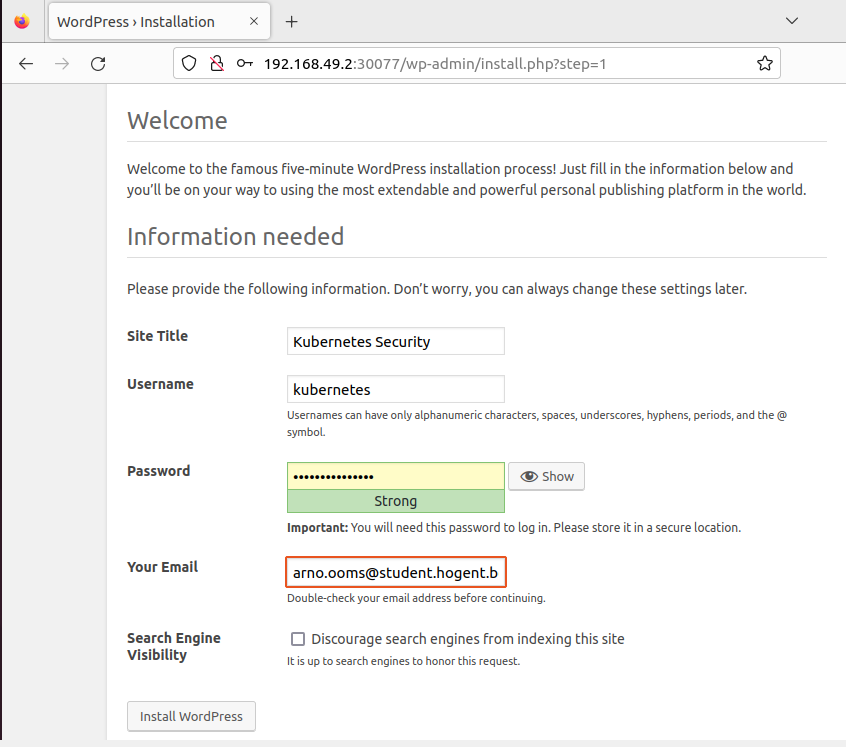
\includegraphics[width=.80\textwidth]{graphics/installeer-wordpress.png}
        \caption{\label{fig:InstallatieKubernetes}Gegevens voor de installatie van Kubernetes.}
    \end{figure} 
\end{flushleft}

\section{Tools en oplossingen}
\subsubsection{Kube-bench}

\paragraph{Stap 1: Installeren}

Haal de job.yaml file van op de officiële documentatie van kube-bench
\begin{lstlisting}[language=tex, caption={Job.yaml halen van documentatie}]
curl -LO -k https://raw.githubusercontent.com/aquasecurity/kube-bench/main/job.yaml
\end{lstlisting}

\paragraph{Stap 2: Uitvoeren}
Na het kopiëren van het bestand is het alleen nodig om dit bestand uit te voeren als een pod met dit commando:
\begin{lstlisting}[language=tex, caption={Job.yaml uitvoeren}]
kubectl apply -f job.yaml
\end{lstlisting}

Verifieer dat het gelukt is met:
\begin{lstlisting}[language=tex, caption={Pods weergeven}]
kubectl get pods
\end{lstlisting}

Kopieer de logs naar een bestand:
\begin{lstlisting}[language=tex, caption={Kopieer de logs naar een bestand}]
kubectl logs '<naam pod>' > kube-bench-logs
\end{lstlisting}

\begin{flushleft}
    \begin{figure}[h]
        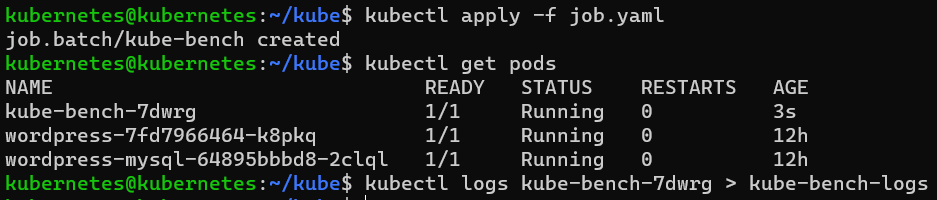
\includegraphics[width=.85\textwidth]{graphics/kube-bench-logs.png}
        \caption{\label{fig:KubebenchLogs}Uitvoeren van Kube-bench}
    \end{figure} 
\end{flushleft}

Bekijk de uivoer van kube-bench met:
\begin{lstlisting}[language=tex, caption={Bekijken uitvoer kube-bench}]
cat kube-bench-logs
\end{lstlisting}


Waarschuwingen en gefaalde testen van de 'control plane security configuration' zijn:
\begin{lstlisting}[language=tex, caption={Warnings en fails kube-bench control plane}]
[INFO] 1 Control Plane Security Configuration
[INFO] 1.1 Control Plane Node Configuration Files
[WARN] 1.1.9 Ensure that the Container Network Interface file permissions are set to 600 or more restrictive (Manual)
[WARN] 1.1.10 Ensure that the Container Network Interface file ownership is set to root:root (Manual)
[FAIL] 1.1.11 Ensure that the etcd data directory permissions are set to 700 or more restrictive (Automated)
[FAIL] 1.1.12 Ensure that the etcd data directory ownership is set to etcd:etcd (Automated)
[FAIL] 1.1.19 Ensure that the Kubernetes PKI directory and file ownership is set to root:root (Automated)
[WARN] 1.1.20 Ensure that the Kubernetes PKI certificate file permissions are set to 600 or more restrictive (Manual)
[WARN] 1.1.21 Ensure that the Kubernetes PKI key file permissions are set to 600 (Manual)
[INFO] 1.2 API Server
[WARN] 1.2.1 Ensure that the --anonymous-auth argument is set to false (Manual)
[FAIL] 1.2.5 Ensure that the --kubelet-certificate-authority argument is set as appropriate (Automated)
[WARN] 1.2.9 Ensure that the admission control plugin EventRateLimit is set (Manual)
[WARN] 1.2.11 Ensure that the admission control plugin AlwaysPullImages is set (Manual)
[WARN] 1.2.12 Ensure that the admission control plugin SecurityContextDeny is set if PodSecurityPolicy is not used (Manual)
[FAIL] 1.2.17 Ensure that the --profiling argument is set to false (Automated)
[FAIL] 1.2.18 Ensure that the --audit-log-path argument is set (Automated)
[FAIL] 1.2.19 Ensure that the --audit-log-maxage argument is set to 30 or as appropriate (Automated)
[FAIL] 1.2.20 Ensure that the --audit-log-maxbackup argument is set to 10 or as appropriate (Automated)
[FAIL] 1.2.21 Ensure that the --audit-log-maxsize argument is set to 100 or as appropriate (Automated)
[WARN] 1.2.22 Ensure that the --request-timeout argument is set as appropriate (Manual)
[WARN] 1.2.29 Ensure that the --encryption-provider-config argument is set as appropriate (Manual)
[WARN] 1.2.30 Ensure that encryption providers are appropriately configured (Manual)
[WARN] 1.2.31 Ensure that the API Server only makes use of Strong Cryptographic Ciphers (Manual)
[INFO] 1.3 Controller Manager
[WARN] 1.3.1 Ensure that the --terminated-pod-gc-threshold argument is set as appropriate (Manual)
[FAIL] 1.3.2 Ensure that the --profiling argument is set to false (Automated)
[INFO] 1.4 Scheduler
[FAIL] 1.4.1 Ensure that the --profiling argument is set to false (Automated)
\end{lstlisting}

De hulpmiddelen die kube-bench biedt zijn:
\begin{lstlisting}[language=tex, caption={Remediations master van kube-bench}]
== Remediations master ==
1.1.9 Run the below command (based on the file location on your system) on the control plane node.
For example, chmod 600 <path/to/cni/files>

1.1.10 Run the below command (based on the file location on your system) on the control plane node.
For example,
chown root:root <path/to/cni/files>

1.1.11 On the etcd server node, get the etcd data directory, passed as an argument --data-dir,
from the command 'ps -ef | grep etcd'.
Run the below command (based on the etcd data directory found above). For example,
chmod 700 /var/lib/etcd

1.1.12 On the etcd server node, get the etcd data directory, passed as an argument --data-dir,
from the command 'ps -ef | grep etcd'.
Run the below command (based on the etcd data directory found above).
For example, chown etcd:etcd /var/lib/etcd

1.1.19 Run the below command (based on the file location on your system) on the control plane node.
For example,
chown -R root:root /etc/kubernetes/pki/

1.1.20 audit test did not run: failed to run: "find /etc/kubernetes/pki/ -name '*.crt' | xargs stat -c permissions=%a", output: "find: /etc/kubernetes/pki/: No such file or directory\nBusyBox v1.35.0 (2022-11-19 10:13:10 UTC) multi-call binary.\n\nUsage: stat [-ltf] [-c FMT] FILE...\n\nDisplay file (default) or filesystem status\n\n\t-c FMT\tUse the specified format\n\t-f\tDisplay filesystem status\n\t-L\tFollow links\n\t-t\tTerse display\n\nFMT sequences for files:\n %a\tAccess rights in octal\n %A\tAccess rights in human readable form\n %b\tNumber of blocks allocated (see %B)\n %B\tSize in bytes of each block reported by %b\n %d\tDevice number in decimal\n %D\tDevice number in hex\n %f\tRaw mode in hex\n %F\tFile type\n %g\tGroup ID\n %G\tGroup name\n %h\tNumber of hard links\n %i\tInode number\n %n\tFile name\n %N\tFile name, with -> TARGET if symlink\n %o\tI/O block size\n %s\tTotal size in bytes\n %t\tMajor device type in hex\n %T\tMinor device type in hex\n %u\tUser ID\n %U\tUser name\n %x\tTime of last access\n %X\tTime of last access as seconds since Epoch\n %y\tTime of last modification\n %Y\tTime of last modification as seconds since Epoch\n %z\tTime of last change\n %Z\tTime of last change as seconds since Epoch\n\nFMT sequences for file systems:\n %a\tFree blocks available to non-superuser\n %b\tTotal data blocks\n %c\tTotal file nodes\n %d\tFree file nodes\n %f\tFree blocks\n %i\tFile System ID in hex\n %l\tMaximum length of filenames\n %n\tFile name\n %s\tBlock size (for faster transfer)\n %S\tFundamental block size (for block counts)\n %t\tType in hex\n %T\tType in human readable form\n", error: exit status 123
1.1.21 audit test did not run: failed to run: "find /etc/kubernetes/pki/ -name '*.key' | xargs stat -c permissions=%a", output: "find: /etc/kubernetes/pki/: No such file or directory\nBusyBox v1.35.0 (2022-11-19 10:13:10 UTC) multi-call binary.\n\nUsage: stat [-ltf] [-c FMT] FILE...\n\nDisplay file (default) or filesystem status\n\n\t-c FMT\tUse the specified format\n\t-f\tDisplay filesystem status\n\t-L\tFollow links\n\t-t\tTerse display\n\nFMT sequences for files:\n %a\tAccess rights in octal\n %A\tAccess rights in human readable form\n %b\tNumber of blocks allocated (see %B)\n %B\tSize in bytes of each block reported by %b\n %d\tDevice number in decimal\n %D\tDevice number in hex\n %f\tRaw mode in hex\n %F\tFile type\n %g\tGroup ID\n %G\tGroup name\n %h\tNumber of hard links\n %i\tInode number\n %n\tFile name\n %N\tFile name, with -> TARGET if symlink\n %o\tI/O block size\n %s\tTotal size in bytes\n %t\tMajor device type in hex\n %T\tMinor device type in hex\n %u\tUser ID\n %U\tUser name\n %x\tTime of last access\n %X\tTime of last access as seconds since Epoch\n %y\tTime of last modification\n %Y\tTime of last modification as seconds since Epoch\n %z\tTime of last change\n %Z\tTime of last change as seconds since Epoch\n\nFMT sequences for file systems:\n %a\tFree blocks available to non-superuser\n %b\tTotal data blocks\n %c\tTotal file nodes\n %d\tFree file nodes\n %f\tFree blocks\n %i\tFile System ID in hex\n %l\tMaximum length of filenames\n %n\tFile name\n %s\tBlock size (for faster transfer)\n %S\tFundamental block size (for block counts)\n %t\tType in hex\n %T\tType in human readable form\n", error: exit status 123
1.2.1 Edit the API server pod specification file /etc/kubernetes/manifests/kube-apiserver.yaml
on the control plane node and set the below parameter.
--anonymous-auth=false

1.2.5 Follow the Kubernetes documentation and setup the TLS connection between
the apiserver and kubelets. Then, edit the API server pod specification file
/etc/kubernetes/manifests/kube-apiserver.yaml on the control plane node and set the
--kubelet-certificate-authority parameter to the path to the cert file for the certificate authority.
--kubelet-certificate-authority=<ca-string>

1.2.9 Follow the Kubernetes documentation and set the desired limits in a configuration file.
Then, edit the API server pod specification file /etc/kubernetes/manifests/kube-apiserver.yaml
and set the below parameters.
--enable-admission-plugins=...,EventRateLimit,...
--admission-control-config-file=<path/to/configuration/file>

1.2.11 Edit the API server pod specification file /etc/kubernetes/manifests/kube-apiserver.yaml
on the control plane node and set the --enable-admission-plugins parameter to include
--enable-admission-plugins=...,AlwaysPullImages,...

1.2.12 Edit the API server pod specification file /etc/kubernetes/manifests/kube-apiserver.yaml
on the control plane node and set the --enable-admission-plugins parameter to include
--enable-admission-plugins=...,SecurityContextDeny,...

1.2.17 Edit the API server pod specification file /etc/kubernetes/manifests/kube-apiserver.yaml
on the control plane node and set the below parameter.
--profiling=false

1.2.18 Edit the API server pod specification file /etc/kubernetes/manifests/kube-apiserver.yaml
on the control plane node and set the --audit-log-path parameter to a suitable path and
file where you would like audit logs to be written, for example,
--audit-log-path=/var/log/apiserver/audit.log

1.2.19 Edit the API server pod specification file /etc/kubernetes/manifests/kube-apiserver.yaml
on the control plane node and set the --audit-log-maxage parameter to 30
or as an appropriate number of days, for example,
--audit-log-maxage=30

1.2.20 Edit the API server pod specification file /etc/kubernetes/manifests/kube-apiserver.yaml
on the control plane node and set the --audit-log-maxbackup parameter to 10 or to an appropriate
value. For example,
--audit-log-maxbackup=10

1.2.21 Edit the API server pod specification file /etc/kubernetes/manifests/kube-apiserver.yaml
on the control plane node and set the --audit-log-maxsize parameter to an appropriate size in MB.
For example, to set it as 100 MB, --audit-log-maxsize=100

1.2.22 Edit the API server pod specification file /etc/kubernetes/manifests/kube-apiserver.yaml
and set the below parameter as appropriate and if needed.
For example, --request-timeout=300s

1.2.29 Follow the Kubernetes documentation and configure a EncryptionConfig file.
Then, edit the API server pod specification file /etc/kubernetes/manifests/kube-apiserver.yaml
on the control plane node and set the --encryption-provider-config parameter to the path of that file.
For example, --encryption-provider-config=</path/to/EncryptionConfig/File>

1.2.30 Follow the Kubernetes documentation and configure a EncryptionConfig file.
In this file, choose aescbc, kms or secretbox as the encryption provider.

1.2.31 Edit the API server pod specification file /etc/kubernetes/manifests/kube-apiserver.yaml
on the control plane node and set the below parameter.
--tls-cipher-suites=TLS_AES_128_GCM_SHA256,TLS_AES_256_GCM_SHA384,TLS_CHACHA20_POLY1305_SHA256,
TLS_ECDHE_ECDSA_WITH_AES_128_CBC_SHA,TLS_ECDHE_ECDSA_WITH_AES_128_GCM_SHA256,
TLS_ECDHE_ECDSA_WITH_AES_256_CBC_SHA,TLS_ECDHE_ECDSA_WITH_AES_256_GCM_SHA384,
TLS_ECDHE_ECDSA_WITH_CHACHA20_POLY1305,TLS_ECDHE_ECDSA_WITH_CHACHA20_POLY1305_SHA256,
TLS_ECDHE_RSA_WITH_3DES_EDE_CBC_SHA,TLS_ECDHE_RSA_WITH_AES_128_CBC_SHA,TLS_ECDHE_RSA_WITH_AES_128_GCM_SHA256,
TLS_ECDHE_RSA_WITH_AES_256_CBC_SHA,TLS_ECDHE_RSA_WITH_AES_256_GCM_SHA384,TLS_ECDHE_RSA_WITH_CHACHA20_POLY1305,
TLS_ECDHE_RSA_WITH_CHACHA20_POLY1305_SHA256,TLS_RSA_WITH_3DES_EDE_CBC_SHA,TLS_RSA_WITH_AES_128_CBC_SHA,
TLS_RSA_WITH_AES_128_GCM_SHA256,TLS_RSA_WITH_AES_256_CBC_SHA,TLS_RSA_WITH_AES_256_GCM_SHA384

1.3.1 Edit the Controller Manager pod specification file /etc/kubernetes/manifests/kube-controller-manager.yaml
on the control plane node and set the --terminated-pod-gc-threshold to an appropriate threshold,
for example, --terminated-pod-gc-threshold=10

1.3.2 Edit the Controller Manager pod specification file /etc/kubernetes/manifests/kube-controller-manager.yaml
on the control plane node and set the below parameter.
--profiling=false

1.4.1 Edit the Scheduler pod specification file /etc/kubernetes/manifests/kube-scheduler.yaml file
on the control plane node and set the below parameter.
--profiling=false

== Summary master ==
37 checks PASS
11 checks FAIL
13 checks WARN
0 checks INFO

\end{lstlisting}

Dit is zijn alleen de resultaten die kube-bench geeft voor de master. 

\subsubsection{KubeLinter}

\paragraph{Stap 1: Installeren}

Voor de installatie voor KubeLinter in deze proof-of-concept is \textit{go} gebruikt. 
Daarvoor is het nodig om go geïnstalleerd te hebben. Dit kan op een linux ubuntu met:
\begin{lstlisting}[language=tex, caption={installeer go}]
snap install go
\end{lstlisting}

Om KubeLinter te installeren is dit commando gebruikt:
\begin{lstlisting}[language=tex, caption={Installeer KubeLinter}]
go install golang.stackrox.io/kube-linter/cmd/kube-linter@latest
\end{lstlisting}

KubeLinter zit nu in de folder: \textit{/home/kubernetes/go/bin/kube-linter}

\paragraph{Stap 2: Uitvoeren}

Deze twee commando's zijn gebruikt om de YAML bestanden te analyseren

\begin{lstlisting}[language=tex, caption={Analyseer YAML bestanden}]
    /home/kubernetes/go/bin/kube-linter lint wordpress-deployment.yaml > wordpresslint
    /home/kubernetes/go/bin/kube-linter lint mysql-deployment.yaml > mysqlLint
\end{lstlisting}


\begin{flushleft}
    \begin{figure}[h]
        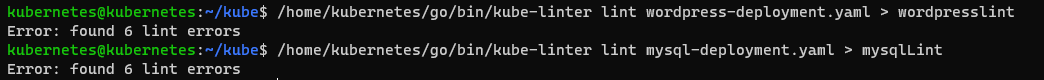
\includegraphics[width=.80\textwidth]{graphics/kubeLinterLinting.png}
        \caption{\label{fig:GebruikKubeLinter}Gebruik KubeLinter.}
    \end{figure} 
\end{flushleft}

Bekijken analyseerde bestanden:
\begin{lstlisting}[language=tex, caption={Bekijk analyse}]
    cat wordpresslint
    cat mysqlLint
\end{lstlisting}

\begin{lstlisting}[language=tex, caption={Analyse wordpress YAML}]
wordpress-deployment.yaml: (object: <no namespace>/wordpress apps/v1, Kind=Deployment) container "wordpress" does not have a read-only root file system (check: no-read-only-root-fs, remediation: Set readOnlyRootFilesystem to true in the container securityContext.)

wordpress-deployment.yaml: (object: <no namespace>/wordpress apps/v1, Kind=Deployment) container "wordpress" is not set to runAsNonRoot (check: run-as-non-root, remediation: Set runAsUser to a non-zero number and runAsNonRoot to true in your pod or container securityContext. Refer to https://kubernetes.io/docs/tasks/configure-pod-container/security-context/ for details.)

wordpress-deployment.yaml: (object: <no namespace>/wordpress apps/v1, Kind=Deployment) container "wordpress" has cpu request 0 (check: unset-cpu-requirements, remediation: Set CPU requests and limits for your container based on its requirements. Refer to https://kubernetes.io/docs/concepts/configuration/manage-resources-containers/#requests-and-limits for details.)

wordpress-deployment.yaml: (object: <no namespace>/wordpress apps/v1, Kind=Deployment) container "wordpress" has cpu limit 0 (check: unset-cpu-requirements, remediation: Set CPU requests and limits for your container based on its requirements. Refer to https://kubernetes.io/docs/concepts/configuration/manage-resources-containers/#requests-and-limits for details.)

wordpress-deployment.yaml: (object: <no namespace>/wordpress apps/v1, Kind=Deployment) container "wordpress" has memory request 0 (check: unset-memory-requirements, remediation: Set memory requests and limits for your container based on its requirements. Refer to https://kubernetes.io/docs/concepts/configuration/manage-resources-containers/#requests-and-limits for details.)

wordpress-deployment.yaml: (object: <no namespace>/wordpress apps/v1, Kind=Deployment) container "wordpress" has memory limit 0 (check: unset-memory-requirements, remediation: Set memory requests and limits for your container based on its requirements. Refer to https://kubernetes.io/docs/concepts/configuration/manage-resources-containers/#requests-and-limits for details.)
\end{lstlisting}

\begin{lstlisting}[language=tex, caption={Analyse MySQL YAML}]
mysql-deployment.yaml: (object: <no namespace>/wordpress-mysql apps/v1, Kind=Deployment) container "mysql" does not have a read-only root file system (check: no-read-only-root-fs, remediation: Set readOnlyRootFilesystem to true in the container securityContext.)

mysql-deployment.yaml: (object: <no namespace>/wordpress-mysql apps/v1, Kind=Deployment) container "mysql" is not set to runAsNonRoot (check: run-as-non-root, remediation: Set runAsUser to a non-zero number and runAsNonRoot to true in your pod or container securityContext. Refer to https://kubernetes.io/docs/tasks/configure-pod-container/security-context/ for details.)

mysql-deployment.yaml: (object: <no namespace>/wordpress-mysql apps/v1, Kind=Deployment) container "mysql" has cpu request 0 (check: unset-cpu-requirements, remediation: Set CPU requests and limits for your container based on its requirements. Refer to https://kubernetes.io/docs/concepts/configuration/manage-resources-containers/#requests-and-limits for details.)

mysql-deployment.yaml: (object: <no namespace>/wordpress-mysql apps/v1, Kind=Deployment) container "mysql" has cpu limit 0 (check: unset-cpu-requirements, remediation: Set CPU requests and limits for your container based on its requirements. Refer to https://kubernetes.io/docs/concepts/configuration/manage-resources-containers/#requests-and-limits for details.)

mysql-deployment.yaml: (object: <no namespace>/wordpress-mysql apps/v1, Kind=Deployment) container "mysql" has memory request 0 (check: unset-memory-requirements, remediation: Set memory requests and limits for your container based on its requirements. Refer to https://kubernetes.io/docs/concepts/configuration/manage-resources-containers/#requests-and-limits for details.)

mysql-deployment.yaml: (object: <no namespace>/wordpress-mysql apps/v1, Kind=Deployment) container "mysql" has memory limit 0 (check: unset-memory-requirements, remediation: Set memory requests and limits for your container based on its requirements. Refer to https://kubernetes.io/docs/concepts/configuration/manage-resources-containers/#requests-and-limits for details.)
\end{lstlisting}

De twee bovenstaande resultaten beschrijven de geanalyseerde bestanden voor de ontplooiing van Wordpress en MySQL.


\subsubsection{Trivy}

\paragraph{Stap 1: Installeren}

Dit is de installatie methode voor Trivy versie 0.41 voor op een Debian/ubuntu. Meerdere installaties kunnen gevonden worden op: \url{https://aquasecurity.github.io/trivy/v0.41/getting-started/installation/}
\begin{lstlisting}[language=tex, caption={Installeren Trivy}]
sudo apt-get install wget apt-transport-https gnupg lsb-release
wget -qO - https://aquasecurity.github.io/trivy-repo/deb/public.key | gpg --dearmor | sudo tee /usr/share/keyrings/trivy.gpg > /dev/null
echo "deb [signed-by=/usr/share/keyrings/trivy.gpg] https://aquasecurity.github.io/trivy-repo/deb $(lsb_release -sc) main" | sudo tee -a /etc/apt/sources.list.d/trivy.list
sudo apt-get update
sudo apt-get install trivy
\end{lstlisting}

\paragraph{Stap 2: Uitvoeren}
\subparagraph{misconfiguratie}
Onderstaand commando scant de configuratie files in de huidige map.
\begin{lstlisting}[language=tex, caption={Scannen configuratie files huidige map}]
trivy config ./
\end{lstlisting}
Het commando geeft veel informatie weer, moeilijk om het te interpreteren. Door het in verschillende categorieën te plaatsen van ernst kan er een duidelijker overzicht gegeven worden. Zo gaat de tool de kritische en hoognodige misconfiguraties weergeven. Aan het begin van de output bij het scannen van de huidige map op fouten in de configuratie staat er een info blokje, een soort samenvatting, over hoeveel testen er geslaagd zijn, hoeveel er gefaald zijn en welke categorie van ernst de gefaalde testen zijn. Deze afbeelding \ref{fig:trivyConfigInfoBlockmysql} is het info blokje bij de output van bovenstaand commando voor het bestand: \textit{mysql-deployment.yaml}. En deze afbeelding \ref{fig:trivyConfigInfoBlockwordpress} voor \textit{wordpress-deployment.yaml}.Per bestand staat er zo een samenvatting.
\begin{flushleft}
    \begin{figure}[h]
        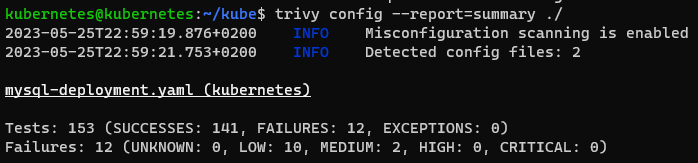
\includegraphics[width=.95\textwidth]{graphics/infoBlockMysqldepl.png}
        \caption{\label{fig:trivyConfigInfoBlockmysql} Info blok van de mysql-deployment.yaml }
    \end{figure} 
\end{flushleft}

\begin{flushleft}
    \begin{figure}[h]
        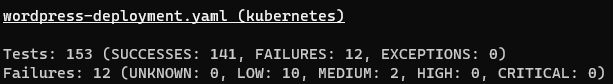
\includegraphics[width=.95\textwidth]{graphics/infoblockwordpressdepl.png}
        \caption{\label{fig:trivyConfigInfoBlockwordpress}Info blok van wordpress-deployment.yaml}
    \end{figure} 
\end{flushleft}

Door deze info zien we dat er geen hoge of kritische misconfiguraties zijn in de bestanden. Er zijn wel \textit{medium failures}. Het is efficiënter en overzichtelijker om onderstaand commando te gebruiken om direct alleen de \textit{medium failures} te bekijken. 
\begin{lstlisting}[language=tex, caption={Medium severity misconfiguraties}]
trivy config --severity=MEDIUM ./
\end{lstlisting}

Afbeelding \ref{fig:trivymediumfailures} toont de twee medium gefaalde testen bij \textit{mysql-deployment.yaml}. Trivy geeft het exacte probleem weer en hoe het opgelost moet worden. Deze twee \textit{medium failures} komen ook voor in het andere bestand \textit{wordpress-deployment.yaml}. 
\begin{flushleft}
    \begin{figure}[h]
        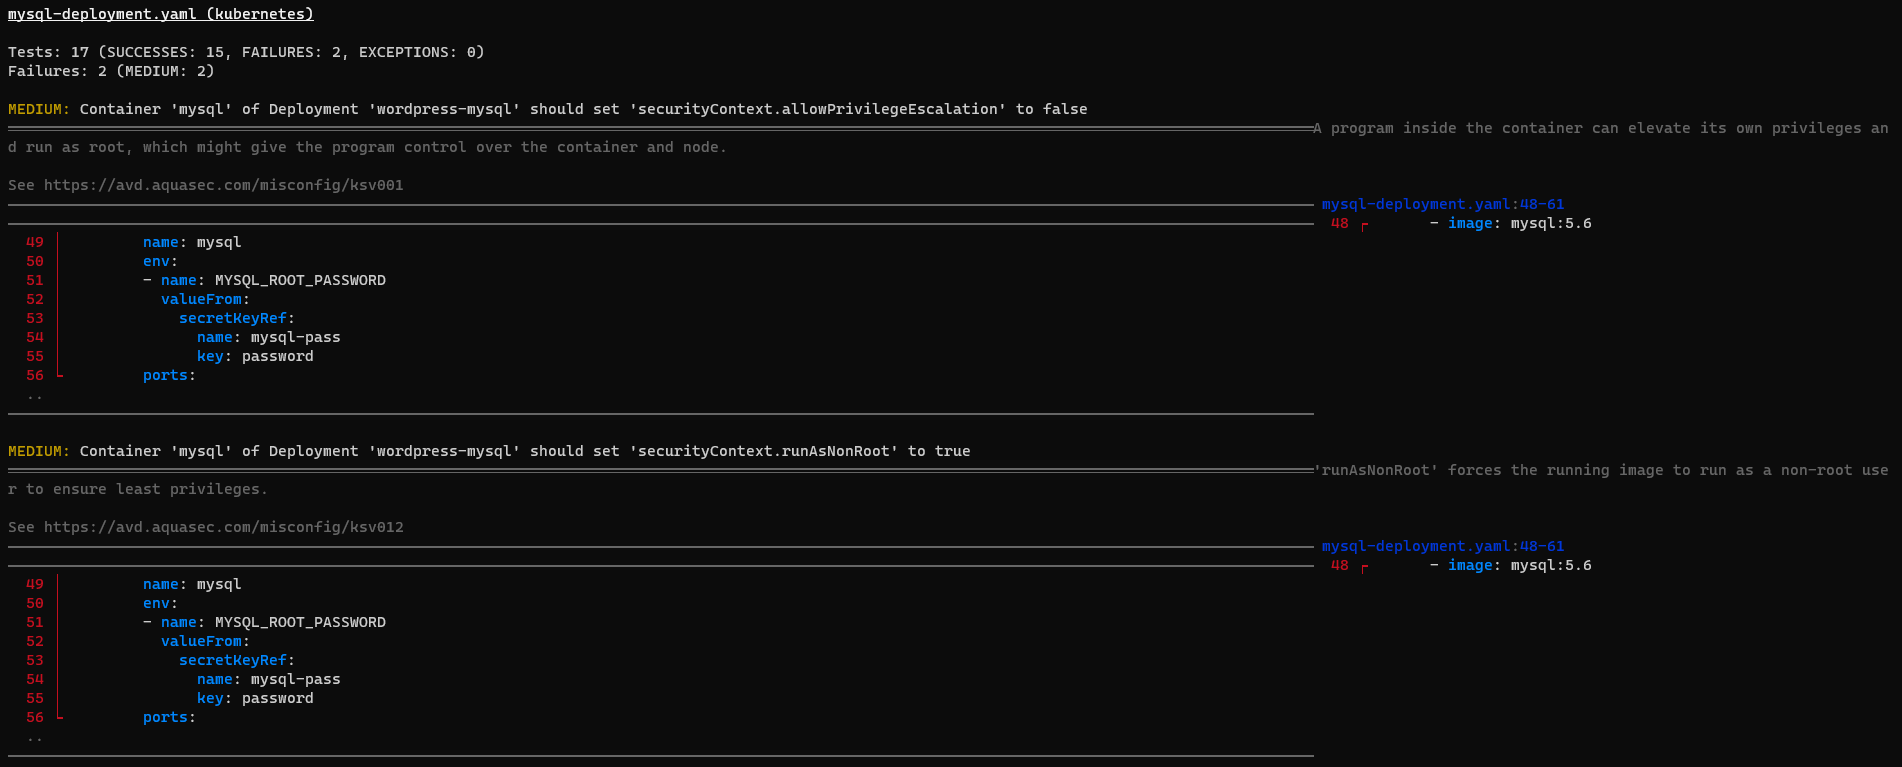
\includegraphics[width=.95\textwidth]{graphics/trivymediumfailures.png}
        \caption{\label{fig:trivymediumfailures} De gefaalde testen op medium ernst van het bestand mysql-deployment.yaml}
    \end{figure} 
\end{flushleft}

\subparagraph{image}

Het scannen van een image:
\begin{lstlisting}[language=tex, caption={Trivy image scanning}]
trivy image [YOUR_IMAGE_NAME]
\end{lstlisting}

De images die in deze proof of concept worden gebruikt zijn: wordpress:4.8-apache en mysql:5.6 dus om deze images te scannen worden deze commando's gebruikt:
\begin{lstlisting}[language=tex, caption={Trivy image scanning wordpress en mysql}]
trivy image wordpress:4.8-apache
trivy image mysql:5.6
\end{lstlisting}

De output bij het scannen van wordpress ziet er zo uit:
\begin{flushleft}
    \begin{figure}[h]
        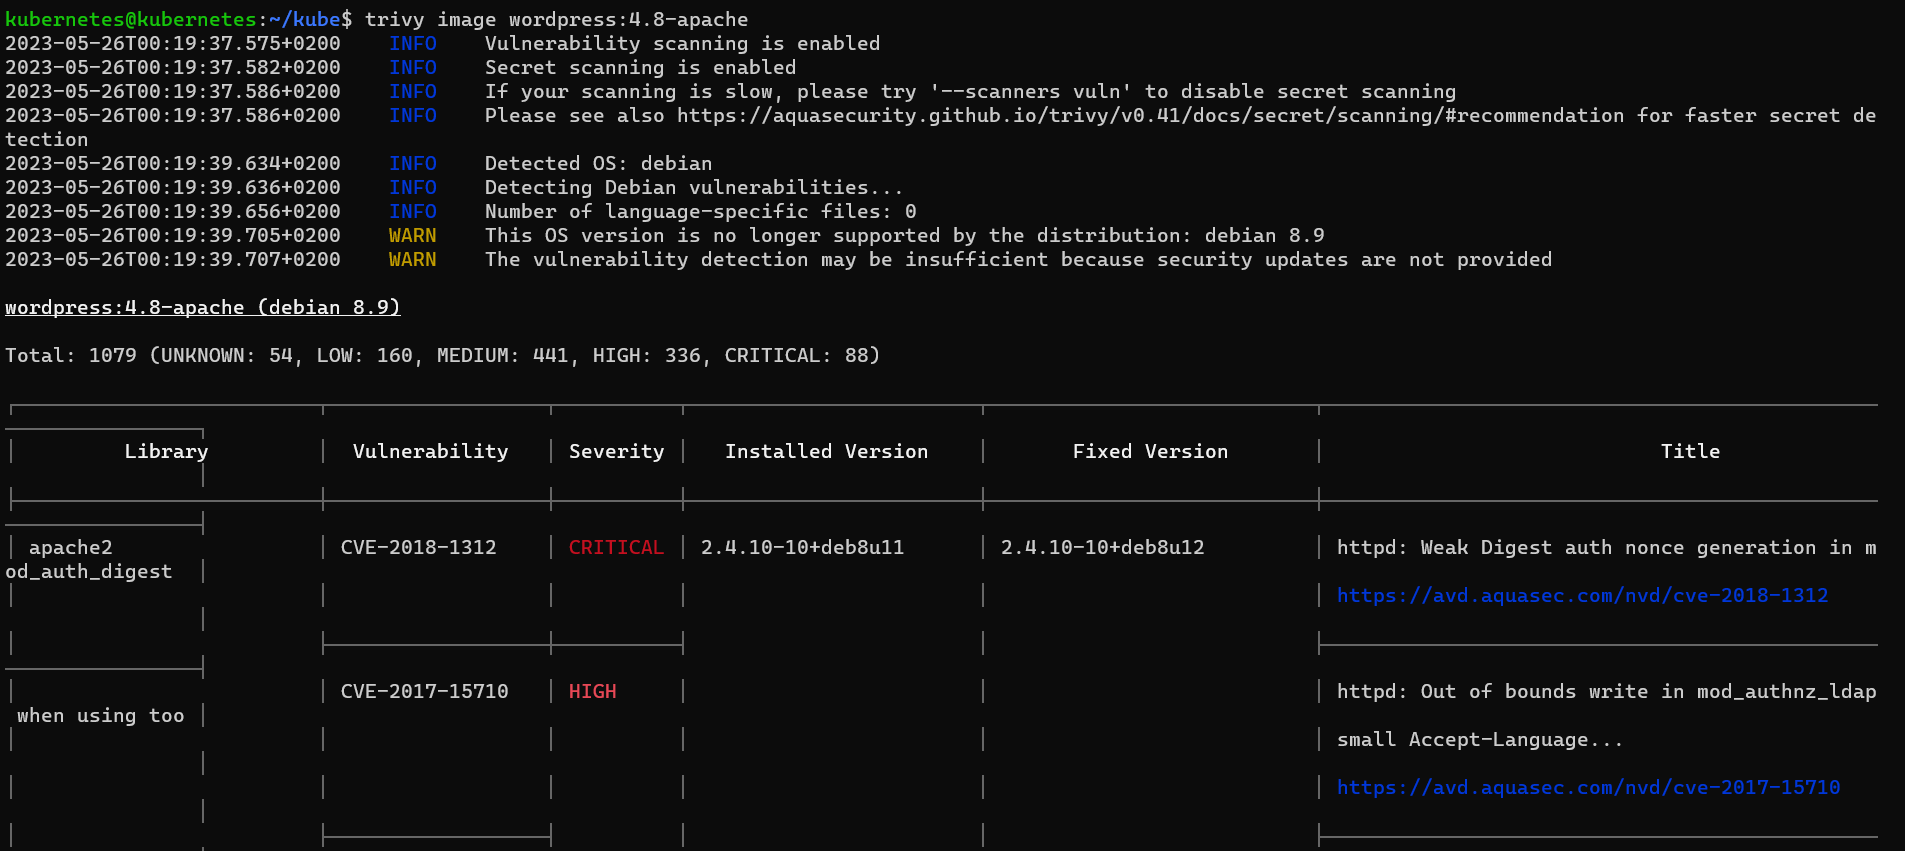
\includegraphics[width=.95\textwidth]{graphics/outputwordpressimagescantrivy.png}
        \caption{\label{fig:TrivyWordpressImageScan}Deze figuur toont de eerste lijnen van de output van het scannen van de wordpress image}
    \end{figure} 
\end{flushleft}

Zoals te zien is op afbeelding \ref{fig:TrivyWordpressImageScan} tonen de eerste 2 lijnen aan dat het scannen van kwetsbaarheden en het scannen van secrets aan staan. Het is mogelijk om de scanners te veranderen en ook bijvoorbeeld de config bij te scannen. Dat kan met dit commando:
\begin{lstlisting}[language=tex, caption={Scannen van config, secret en kwetsbaarheden binnen wordpress image}]
trivy image --scanners config,secret,vuln wordpress:4.8-apache
\end{lstlisting}

Wat er ook te zien is op de image scan zijn de totale aantal scans: 1079. 54 daarvan zijn onbekend, 160 zijn laag, 441 medium, 336 hoog en 88 kritisch. Om alleen de kritische weer te geven is dat mogelijk met dit commando:
\begin{lstlisting}[language=tex, caption={Scannen van config, secret en kwetsbaarheden binnen wordpress image met kritische ernst}]
trivy image --severity=CRITICAL --scanners config,secret,vuln wordpress:4.8-apache
\end{lstlisting}

In afbeelding \ref{fig:TrivyWordpresCriticalScan} is te zien dat de image versie 2.4.10 van apache2 gebruikt. Die versie van apache2 heeft een kwetsbaarheid van in de CVE database \textit{CVE-2018-1312}. 
\begin{flushleft}
    \begin{figure}[h]
        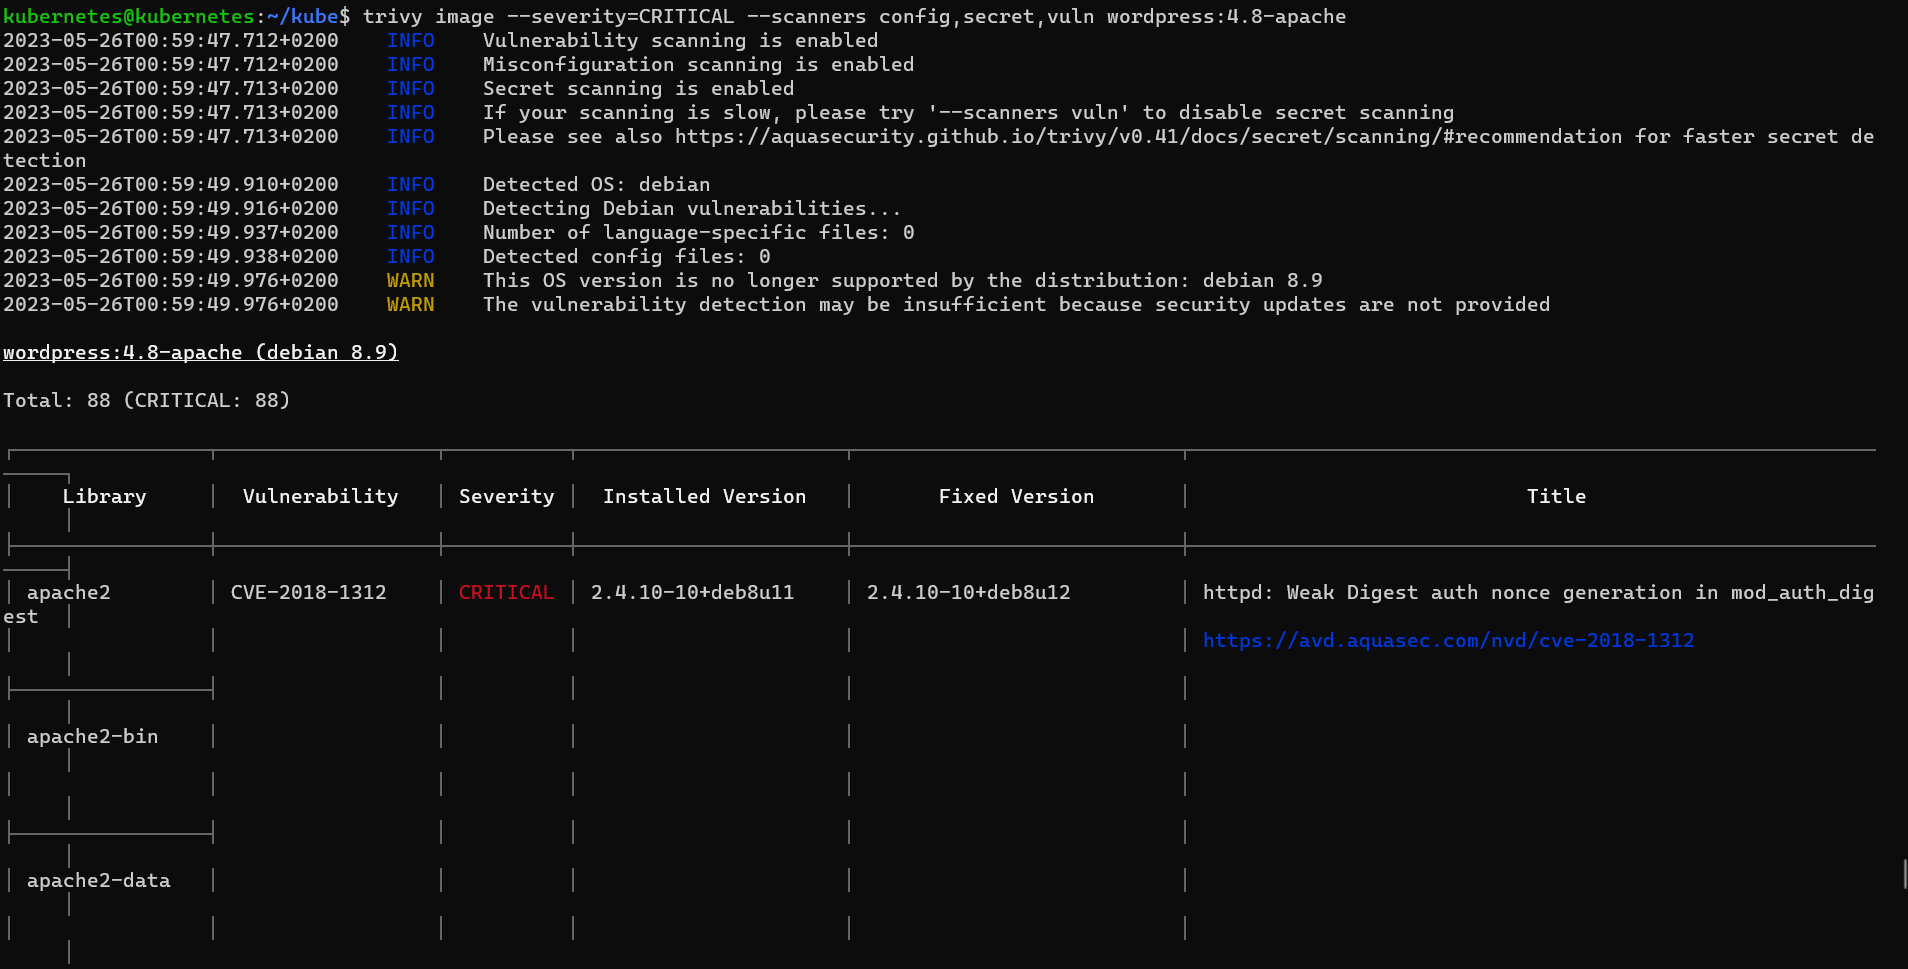
\includegraphics[width=.95\textwidth]{graphics/trivyapachekritisch.png}
        \caption{\label{fig:TrivyWordpresCriticalScan}De output van de kritische kwesbaarheden, configs en secrets. Daaronder is er een kritische kwetsbaarheid te zien van apache2.}
    \end{figure} 
\end{flushleft}

\subparagraph{SBOM}
Binnen de supply chain helpt Trivy met de beveiliging aan de hand van een SBOM (Software Bill Of Materials). Trivy kan een SBOM genereren in het CycloneDX formaat. CycloneDX kan zowel SBOM als BOV (Bill of Vulnerabilities) voorstellen. Standaard staat --format cyclonedx voor SBOM en neemt kwetsbaarheden niet op in de CycloneDX uitvoer. Het volgend commando toont hoe de SBOM van de image \textit{wordpress:4.8-apache} gegenereert word en gescant word.
\begin{lstlisting}[language=tex, caption={SBOM scannen en analyseren met Trivy}]
trivy image --format cyclonedx --output result.json wordpress:4.8-apache
trivy sbom spdx.json
\end{lstlisting}

Als het doel is om kwetsbaarheden op te nemen is het mogelijk om het scannen op kwetsbaarheden in te schakelen via \textit{--scanners vuln}.
\begin{lstlisting}[language=tex, caption={SBOM scannen en analyseren met Trivy en kwetsbaarheden inschakelen}]
trivy image --scanners vuln --format cyclonedx --output result.json wordpress:4.8-apache
trivy sbom spdx.json
\end{lstlisting}

Het is ook mogelijk om een SBOM te creëren in het formaat SPDX \footnote{https://spdx.dev/wp-content/uploads/sites/41/2020/08/SPDX-specification-2-2.pdf} en SPDX in json.


\subparagraph{Cluster scanning}
Nog een functie die Trivy biedt is het scannen van Kubernetes cluster. Het volgende commando scant de volledige cluster en genereert een rapport in de vorm van een samenvatting. In afbeelding \ref{fig:TrivyKubernetesClusterScan} is de output van de workload beoordeling te zien. 
\begin{lstlisting}[language=tex, caption={Scannen Kubernetes cluster met Trivy}]
trivy k8s --report=summary cluster
\end{lstlisting}

\begin{flushleft}
    \begin{figure}[h]
        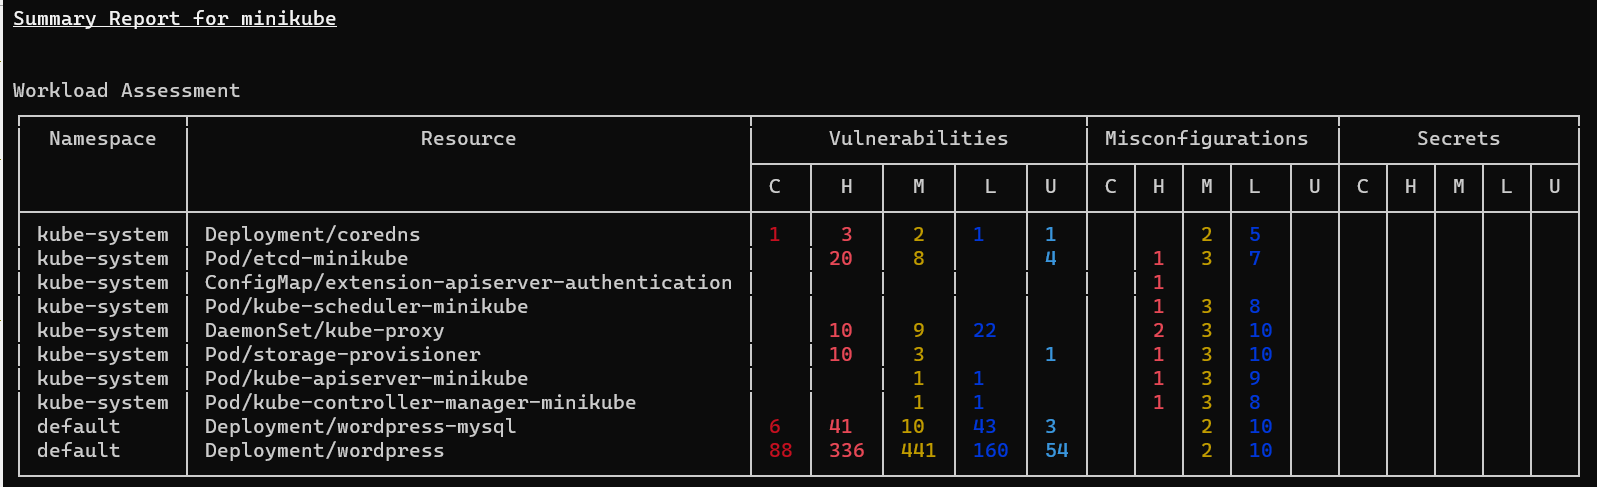
\includegraphics[width=.95\textwidth]{graphics/outputK8SscanTrivy.png}
        \caption{\label{fig:TrivyKubernetesClusterScan}Dit is de beoordeling van de workload van Trivy voor de kubernets scan.}
    \end{figure} 
\end{flushleft}

Trivy doet bij een Kubernetes scan ook direct een image scan van de images dat Trivy heeft gedetecteerd en daarbuiten geeft de tool info voor RBAC en infra. Het is ook mogelijk om verschillende rapporten te maken op basis van de \textit{compliance}. Afbeelding \ref{fig:complianceRestricted} is het resultaat van een rapport van de kubernetes cluster op basis van de \textit{compliance} van beperkte beveiligingsstandaarden van een pod of ook wel \textit{Pod Security Standards, Restricted}.  

\begin{flushleft}
    \begin{figure}[h]
        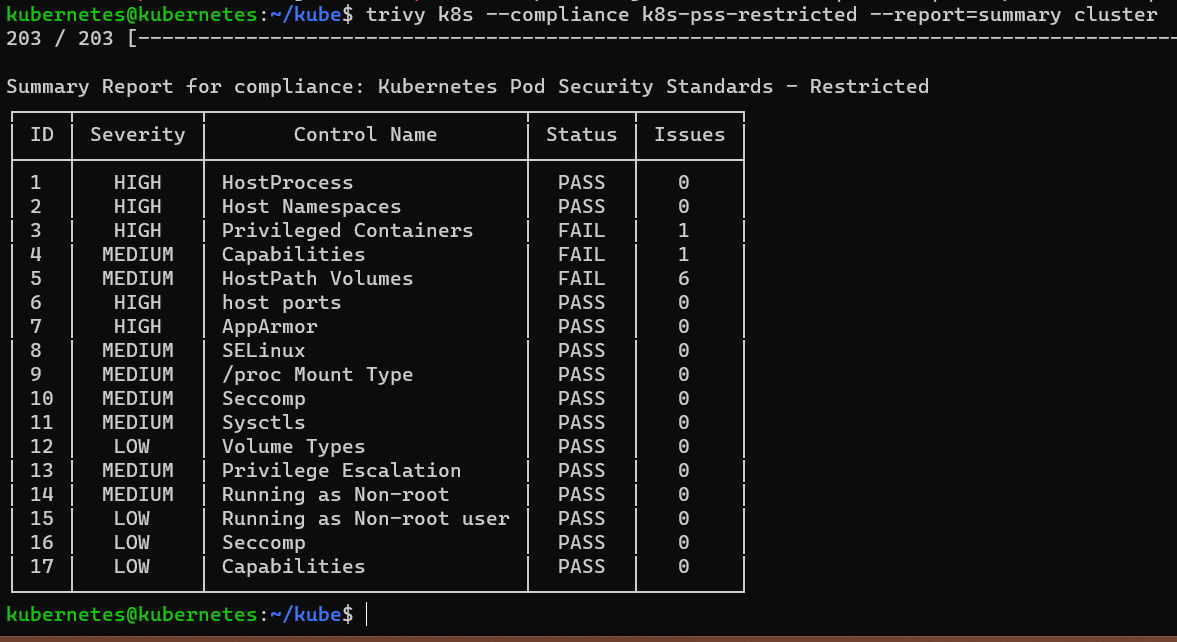
\includegraphics[width=.95\textwidth]{graphics/complianceRestricted.png}
        \caption{\label{fig:complianceRestricted}De output van de \textit{compliance} Pod Security Standards - Restricted}
    \end{figure} 
\end{flushleft}



\subsubsection{OPA - OPA gatekeeper}

\paragraph{Stap 1: Installeren}
Admin permissies geven aan de gebruiker kubernetes voor de installatie van OPA:
\begin{lstlisting}[language=tex, caption={Installatie OPA}]
  kubectl create clusterrolebinding cluster-admin-binding \
--clusterrole cluster-admin \
--user kubernetes
\end{lstlisting}

Ontplooien van OPA in cluster:
\begin{lstlisting}[language=tex, caption={OPA ontplooien in cluster}]
kubectl apply -f https://raw.githubusercontent.com/open-policy-agent/gatekeeper/master/deploy/gatekeeper.yaml
\end{lstlisting}

\paragraph{Stap 2: Uitvoeren}

Nu OPA gatekeeper op de cluster staat, is het mogelijk om beleidsregels toe te passen. Onderstaand commando haalt de beleidsregel op en voert het uit:
\begin{lstlisting}[language=tex, caption={Beleidsregels OPA ophalen}]
kubectl apply -f https://raw.githubusercontent.com/open-policy-agent/gatekeeper-library/master/library/pod-security-policy/allow-privilege-escalation/template.yaml
\end{lstlisting}

\textit{Wordpress-deployment.yaml} bestand wordt aangepast om de beleidsregel te testen.
\begin{itemize}
    \item voeg het veld securityContext toe in het bestand
    \item Voeg daaronder toe: \textit{allowPriviligeEscalation: true}
\end{itemize}

Het stukje code van \textit{wordpress-deployment.yaml} zal er dan zo uit zien:
\begin{lstlisting}[language=tex, caption={Stukje van \textit{wordpress-deployment.yaml} met securityContext}]
volumeMounts:
- name: wordpress-persistent-storage
  mountPath: /var/www/html
securityContext:
  allowPriviligeEscalation: true
volumes:
- name: wordpress-persistent-storage
  persistentVolumeClaim:
    claimName: wp-pv-claim
\end{lstlisting}

Pas de nieuwe aanpassingen toe:
\begin{lstlisting}[language=tex, caption={Wijzigingen aanbrengen}]
kubectl apply -k ./
\end{lstlisting}

Het resultaat wijst op een \textit{invalid request}:
\begin{flushleft}
    \begin{figure}[h]
        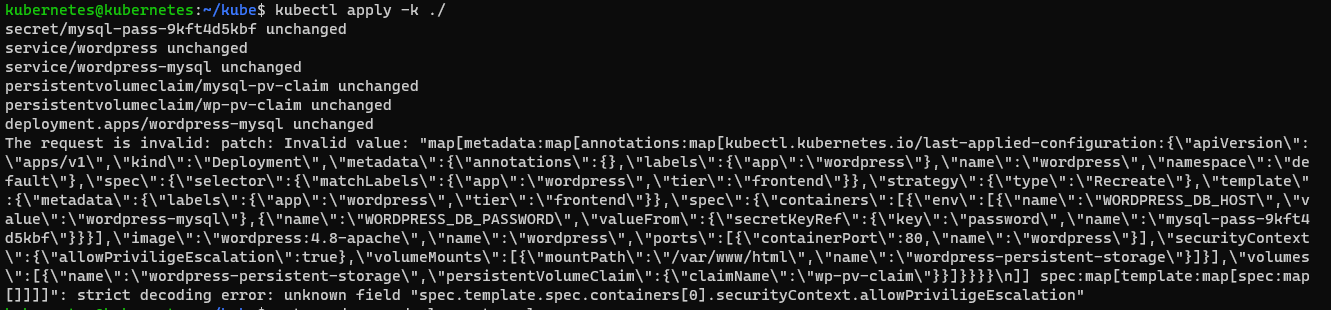
\includegraphics[width=.95\textwidth]{graphics/invalidRequest.png}
        \caption{\label{fig:invalidRequest}De output van het toepassen van de beleidsregel van OPA gatekeeper}
    \end{figure} 
\end{flushleft}

\subsubsection{Kube-hunter}

\paragraph{Stap 1: Installeren}
Onderstaande commando's zijn gebruikt om kube-hunter te installeren.
\begin{lstlisting}[language=tex, caption={Kube-hunter installeren}]
git clone https://github.com/aquasecurity/kube-hunter.git
cd ./kube-hunter
pip install -r requirements.txt
\end{lstlisting}

\paragraph{Stap 2: Uitvoeren}
Uitvoeren kan met: 
\begin{lstlisting}[language=tex, caption={kube-hunter uitvoeren}]
    python3 kube_hunter
\end{lstlisting}

Het resultaat is:
\begin{flushleft}
    \begin{figure}[h]
        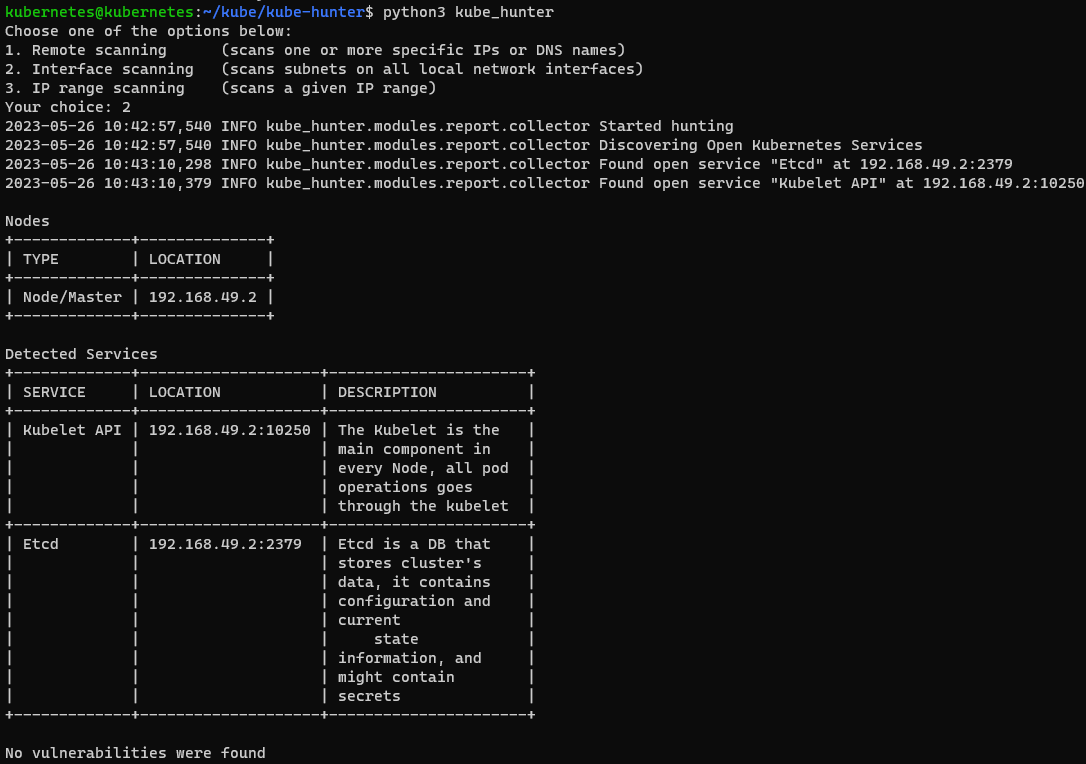
\includegraphics[width=.95\textwidth]{graphics/kubeHunterMachineOutput.png}
        \caption{\label{fig:invalidRequest}De output van kube-hunter geïnstalleerd met pip}
    \end{figure} 
\end{flushleft}

Om kube-hunter als pod in de cluster te draaien zijn deze commando's gebruikt:
\begin{lstlisting}[language=tex, caption={Kube-hunter in een pod draaien}]
    git clone https://github.com/aquasecurity/kube-hunter.git
    cd ./kube-hunter
    kubectl create -f ./job.yaml
\end{lstlisting}

Na het creëren van de pods krijgen de pods een error:
\begin{flushleft}
    \begin{figure}[h]
        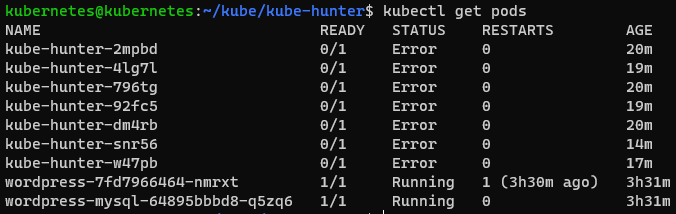
\includegraphics[width=.95\textwidth]{graphics/podsError.png}
        \caption{\label{fig:kube-hunterFail}De output van kube-hunter \textit{job.yaml}}
    \end{figure} 
\end{flushleft}

De logs van zo een pod is dit:
\begin{flushleft}
    \begin{figure}[h]
        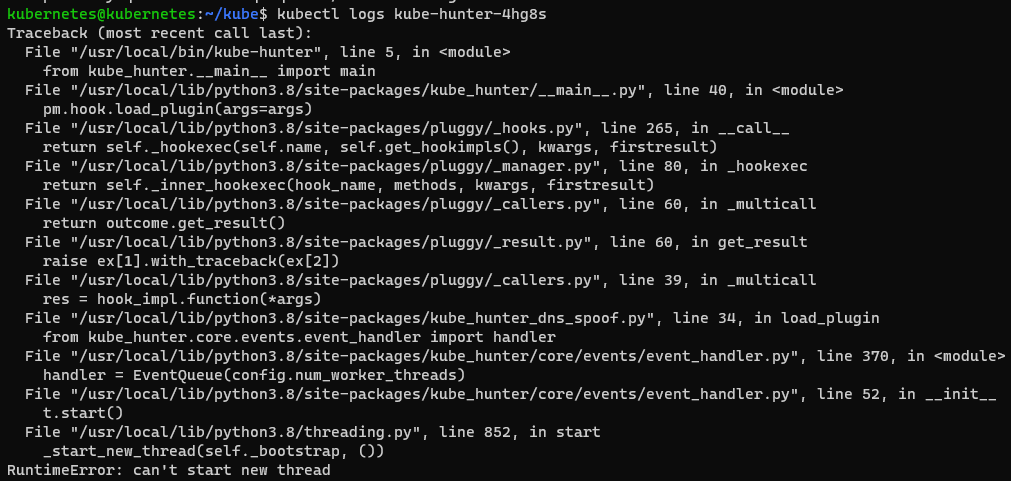
\includegraphics[width=.95\textwidth]{graphics/errorPods.png}
        \caption{\label{fig:kube-hunterFail}Logs van error pod}
    \end{figure} 
\end{flushleft}


    